\section{Jakub Brzeźniak}
\label{sec:jbrzezniak}

\begin{figure}
    \centering
    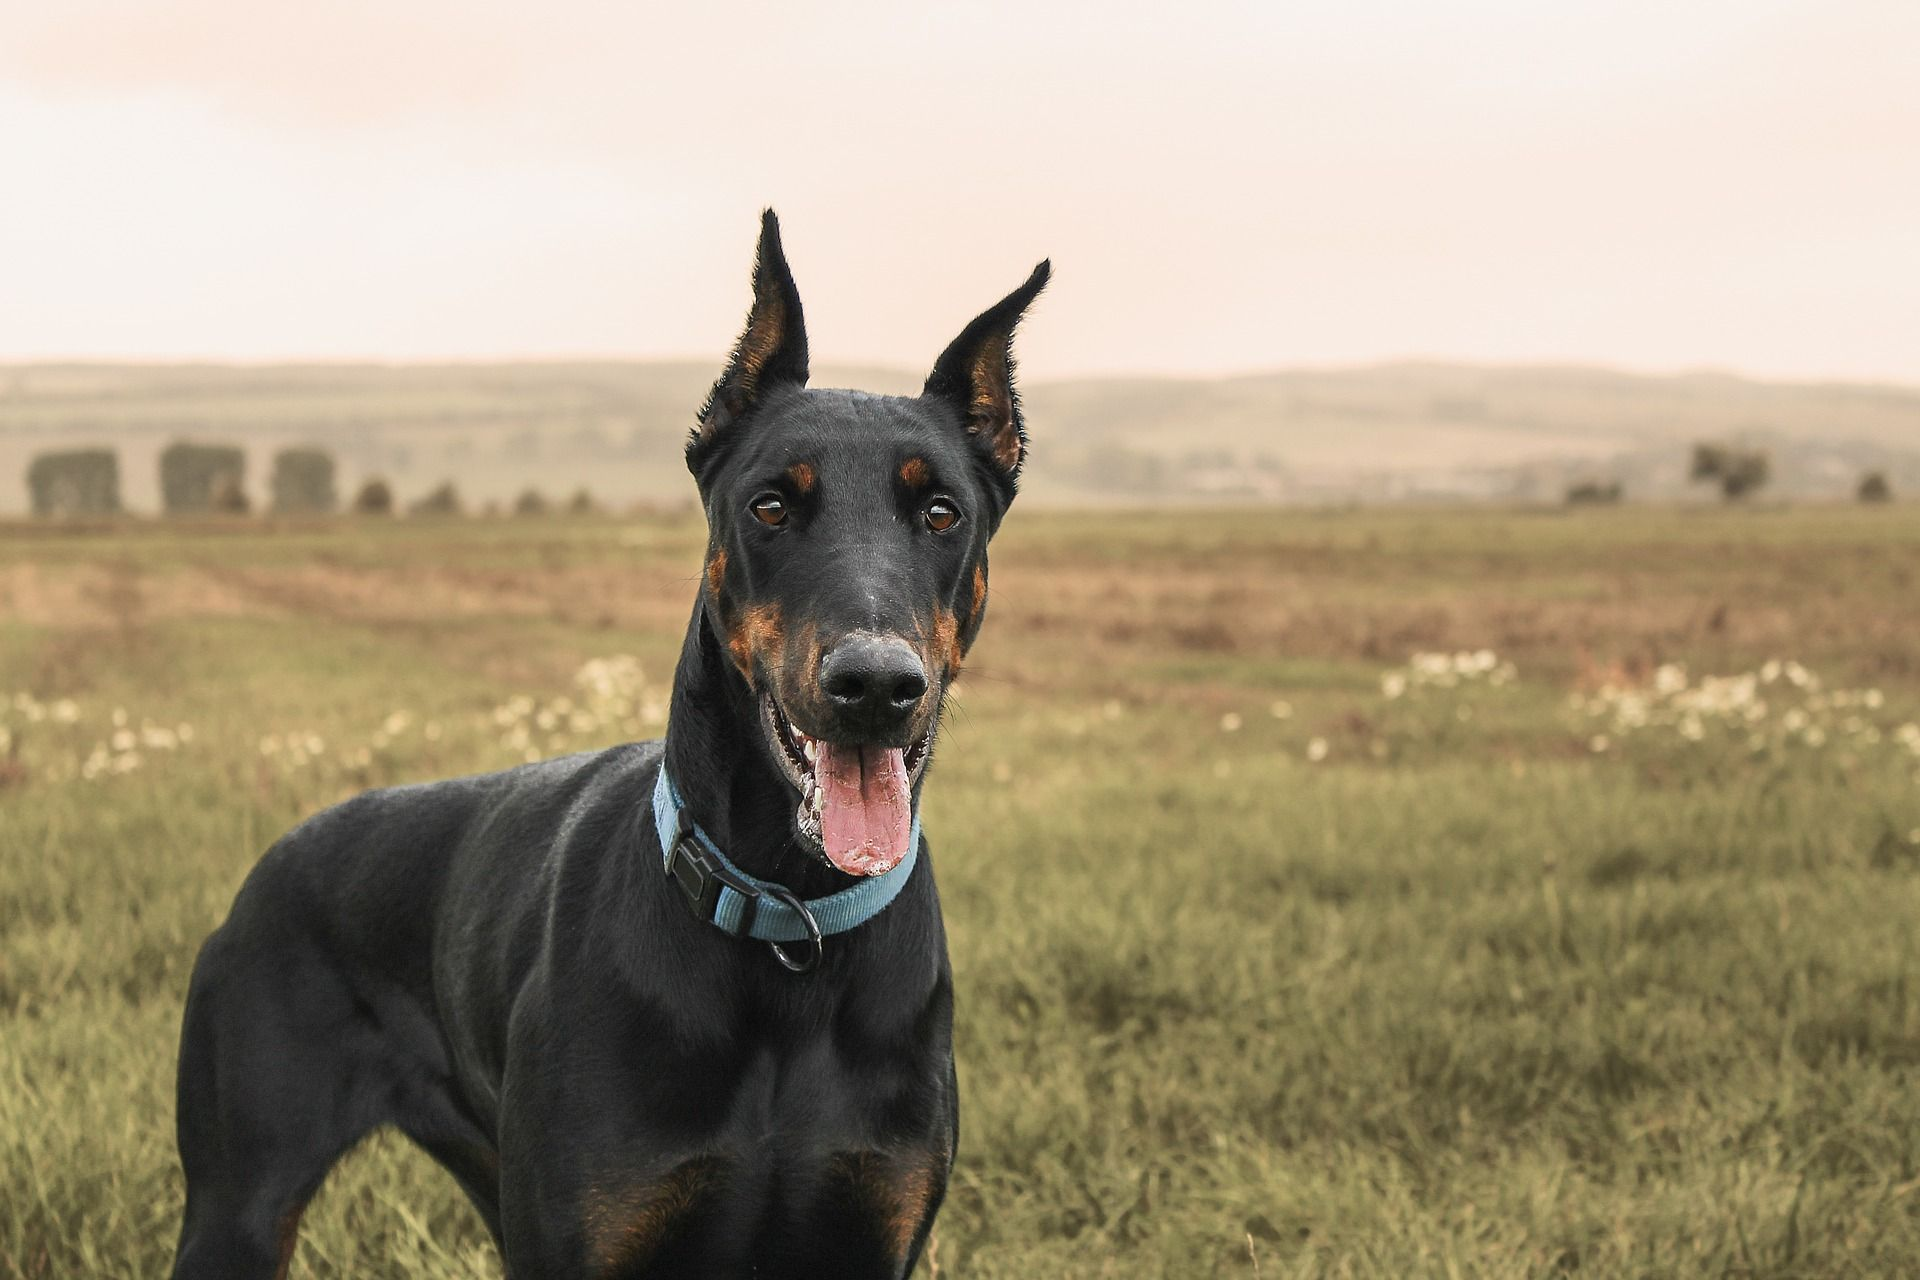
\includegraphics{pictures/doberman.jpg}
    \caption{Wybralem zdjecie dobermana}
\end{figure}



\textbf{Przykładowa macierz 4x4:}
\begin{table}[h]
\centering
\begin{tabular}{|c|c|c|}
\hline
14 & 67 & 1 \\ \hline
68 & 32 & 2  \\ \hline
-43 & 21  & -23  \\ \hline
\end{tabular}
\end{table}



\textbf{wielcy polacy}
\begin{enumerate}
    \item mariusz pudzianowski
    \item piotr zyla
    \item tomasz karolak
\end{enumerate}

\textbf{mniejsi polacy}
\begin{itemize}
    \item ja
    \item moj kolega tomek
    \item moj kolega maciek
\end{itemize}



\textbf{podstawowe wzory}
\[(a+b)^2=a^2+2ab+b^2\]
\newpage
\textbf{rasa psa zaliczana do grupy \textcolor{blue}{pinczerów}. Krajem pochodzenia tej rasy są Niemcy. W klasyfikacji FCI zaliczona została do grupy 2 (pinczery i sznaucery, molosy, szwajcarskie psy górskie i do bydła, pozostałe rasy), sekcji 1 \textit{pinczery i sznaucery}. Psy tej rasy celem uzyskania kwalifikacji hodowlanych muszą być poddane próbom pracy. Typ wilkowaty}
\textbf{Rasa wywodzi się z \textcolor{red}{Niemiec}, nazwa pochodzi od nazwiska Karla Friedricha Louisa Dobermanna}
